% Software License Agreement
%
% Author    Chris Bogdon <cbogdon@clearpathrobotics.com>
% Copyright (c) 2015, Clearpath Robotics, Inc., All rights reserved.
%
% Redistribution and use in source and binary forms, with or without modification, is
% not permitted without the express permission of Clearpath Robotics.


\documentclass[]{clearpath-latex/clearpath-manual}
\graphicspath{{gen/}}
\usepackage{multirow}
\usepackage{gensymb}
\usepackage{dcolumn}
\usepackage{colortbl}
\usepackage{array}
\usepackage{hyperref}
\usepackage{fancyhdr}
\usepackage{pdfpages}
\pagestyle{fancyplain}
\lfoot{Rev. 2.0.0}
\rfoot{Warthog UGV}
\lhead{}
\chead{}
\rhead{}
\renewcommand{\headrulewidth}{0pt}


\begin{document}

\manualcover{cover-page.pdf}
\tableofcontents




\section{Introduction}
Clearpath Robotics Warthog is a rugged, all-terrain unmanned ground vehicle capable of travelling on land and in water.  Warthog fully supports Robot Operating System (ROS), and can be equipped with a variety of payloads. Payloads such as sensors and manipulators to accommodate a wide range of robotics applications in mining, agriculture, and environmental monitoring. This guide contains information about the setup, safe operation, and maintenance of your Warthog.  Please read the entire manual and safety warnings prior to operating the Warthog.

\subsection{What's Included}

Included with each Warthog are the following:

\begin{itemize}[nolistsep]
  \item 1x Warthog UGV
  \begin{itemize}
    \item{Onboard computer}
    \item{User Panel with power, Ethernet, Serial(RS232) and USB connectivity}
    \item{48V Lead Acid/Lithium Battery Pack}
    \item{Battery Charger}
  \end{itemize}
  \item 1x Futaba Remote Control (R/C)
  \item 1x Warthog User Manual
  \item 1x Wireless Stop Remote
\end{itemize}



\pagebreak[4]
\subsection{Hardware Overview}

Please see \autoref{Warthog_overview} for a view of some of Warthog's key external-facing features.

\begin{figure}[h]
  \centering
  \includegraphics[width=1\linewidth]{graphics/Warthog_Drawing_Labeled.png}
  \caption{Warthog Hardware Overview}
  \label{Warthog_overview}
\end{figure}





\pagebreak[4]
\subsubsection{Battery Charger}
Please see Appendix 1 for information about the provided charger.

\subsubsection{Bilge Pumps}\label{bilgepumps}
The Warthog has two bilge pumps, with one situated in each of the drive units underneath the motor.

The bilge pumps are used to remove water from the main chassis and drive units during operation in water. If the water level inside the drive unit exceeds a predetermined level, the pumps will remain on, otherwise they will shut off. During prolonged use in water, some water may appear in the drive unit. This is normal and acceptable.

The Warthog comes equipped with a bilge pump in each of the side drive units. These pumps are used to remove any water coming into the main chassis or drive units during operation in water. If water exceeds a certain level, the pumps will activate automatically and run until the water has receded to a safe level. During prolonged use in water, it is normal and acceptable to see water appear in the drive units. 

%% Picture of bilge pumps

Each drive unit has a bilge pump outlet on the side of the drive unit. No obstructions should be placed in front of or around this area. Obstruction of water flow may result in damage to the internal electrical components and loss of function in the Warthog.

\subsubsection{User Panel}\label{userarea}

The top plate provides access to user power, as well as USB, serial, and ethernet ports. These connections can be used to power and communicate with your payloads. The USB 3.0 and ethernet  ports are connected directly to the onboard PC. To connect a device to the onboard network, it's suggested to give it a static IP in the \lstinline{192.168.131.x} subnet, avoiding IPs in use by the following pre-existing devices:

\bgroup
\def\arraystretch{1.2}%
\begin{table}[h]
  \centering
  \begin{tabular}{>{\columncolor{lightgrey}}>{\raggedright}m{.3\textwidth} p{.65\textwidth}} \hline

  192.168.131.1 & Onboard PC (all ports, br0 network interface). \\ \hline

  192.168.131.2 & Ethernet-connected MCU. \\ \hline

  192.168.131.20 & Primary LIDAR (optional). \\ \hline

  192.168.131.21 & Secondary LIDAR (optional). \\ \hline

  \end{tabular}
\newline
\caption{Warthog Onboard Network Devices}
\label{netdevs}
\end{table}
\egroup

For more information on electrical integration, please see \autoref{electrical} on page \pageref{electrical}.

\pagebreak[4]


\subsubsection{Payload Integration Area}

All payloads should be mounted to the central chassis when traversing through water to prevent rolling. The primary payload of the unit should be placed on the central chassis. If necessary loading can be placed on the drive units however payloads should not exceed 50 lbs on each drive unit.

For more information and guidance on mounting payload structures on top of Warthog, please refer to \autoref{mechanical} on page \pageref{mechanical}.


\pagebreak[4]
\subsection{Technical Specifications}

Key specifications of Warthog are shown in \autoref{systemspecs}.

\bgroup
\def\arraystretch{1.2}%
\begin{table}[h]
  \centering
  \begin{tabular}{>{\columncolor{lightgrey}}>{\raggedright}m{.30\textwidth} p{.70\textwidth}} \hline

  External Dimensions (L x W x H) & 1.52 x 1.38 x 0.83 m (4.9 x 4.5 x 2.72 ft ) \\ \hline
  Base Weight & 280 kg (551 lbs) \\ \hline
  Ground Clearance & 254 mm (10 in) \\ \hline
  Max Payload  &  272 kg (600 lbs)   \\ \hline
  Max Incline & 35-45° (dependent on payload) \\ \hline
  Max Speed  &  18 km/h (11 mph) \\ \hline
  Suspension & Geometric Passive Articulation \\ \hline
  Drive Configuration &  4x4 Skid Steer \\ \hline
  Operating Environment  &  Outdoor \\ \hline
  Traction & 24" Argo tire (24" Turf tire or 12" wide Quad Track System optional) \\ \hline
  Battery Chemistry & AGM sealed lead acid or Li-ion \\ \hline
  Capacity &  105 Ah at 48 V \\ \hline
  Nominal Run Time & Lead acid: 2.5 hrs, Li-ion: 6 hrs \\ \hline
  Charge Time &  6 to 8 Hours \\ \hline
  User Power & 12 V, 24 V and 48 V Fused at 10A \\ \hline
  Control Modes & Remote control, computer controlled velocity commands, indoor/outdoor autonomy packages \\ \hline
  Feedback & Battery voltage, motor currents, wheel odometry, control system status, temperature, safety status \\ \hline
  Communication &  Ethernet, USB, Remote Control, Wi-Fi \\ \hline
  Drivers and APIs  &  Packaged with ROS Melodic (includes RViz, Gazebo support), Matlab API available \\ \hline

  \end{tabular}
\newline
\caption{Warthog System Specifications}
\label{systemspecs}
\end{table}
\egroup


\section{Safety Considerations}

Warthog is a powerful, heavy, fast moving robotic platform. Please read the following safety information carefully.

\subsection{General Warnings}

For the safety of yourself and others, always conduct initial experiments and software development with the motors not engaged.  Whenever the robot is not being operated and the motors are engaged, keep it in a stop state.  Do not ride on the vehicle, it can accelerate and brake quickly.

When starting out, favour slower wheel speeds. Warthog's control loops can accurately maintain velocities as low as 0.1 m/s. Operating at such speeds will give you more time to react if things don’t go quite as you expect.

When enabling the system using the Start button on the wireless remote, be sure to stand well back from the Warthog. User code running on the Warthog may still be trying to command the motors, and this can result in sudden and unexpected movement of the vehicle. Be prepared to stop the system again using the wireless remote.

\subsection{Safety Features}
The following risk reduction measures have been incorporated into the base Warthog UGV:

\begin{itemize}[nolistsep]
  \item Circuit protection in the form of fuses, as shown in system electrical schematics
  \item Mechanical enclosure of components that present electrical, thermal or mechanical hazards
  \item Use of suitable components for critical functions
  \item Mechanical brakes mounted to each traction motor shaft to reduce likelihood of unintended vehicle motion
  \item Motor temperature feedback and monitoring to prevent faults due to motor over-temperature
  \item Closed-loop motor control with encoder feedback to reduce likelihood of unintended vehicle motion
  \item Bilge pumps to prevent electrical faults due to water ingress
  \item Use of finger-safe electrical connectors where live electrical components are externally accessible to users
  \item Main battery disconnect to reduce likelihood of harm during assembly, transportation and maintenance
  \item Brightly-coloured, contrasting surface coatings and lighting to increase visibility and avoidability
  \item Computer-to-microcontroller watchdog timer with stop function to prevent hazards due to computer failures
  \item Emergency stop actuators mounted on the vehicle to bring it to a safe state
  \item Remote (wireless) emergency stop pendant to bring the vehicle to a safe state
  \item Remote emergency stop system to bring vehicle to a safe state if connection to pendant is lost
  \item Remote controls allow operator to physically separate themselves from vehicle
  \item Mechanical transmissions include disconnection levers that allow motors to be physically disconnected from wheels to prevent unintended vehicle motion
\end{itemize}

\subsection{Risk}
The following residual risks exist and must be recognized and accepted by integrators and users:

\begin{itemize}[nolistsep]
  \item It is possible for a single fault condition to result in loss of safety functions including stop function
  \item It is possible that the loss of safety functions will go undetected by the vehicle control system
  \item The vehicle is incapable of detecting obstacles in its environment and will not intervene to avoid collisions with persons or animals in its path
  \item When drivetrain levers are in the “neutral” position the vehicle’s mechanical brakes are not connected to the wheels; the vehicle may roll on a grade or in response to an applied force (see section 3.7)
  \item The vehicle is capable of high acceleration and the area around the robot should always be considered a hazard zone, regardless of “current” vehicle speed
  \item There are many exposed, live electrical terminals and conductors inside the robot
  \item Manipulation of the drivetrain disconnection levers requires reaching down into the vehicle in an awkward manner that could result in injury, especially if the vehicle moves unexpectedly during manipulation
  \item In the case of the bilge pumps blowing the 24V fuse, the wireless E-stop will activate due to loss of power, which will turn off the motors and pumps; this could potentially cause damage or danger
  \item The external suspension linkage at the back of the vehicle presents an unguarded pinch/crush hazard
  \item External access panel and doors are not interlocked; electrical components may be live and accessible
  \item Certain accessible internal surfaces such as motor housing may become dangerously hot during operation
\end{itemize}


\subsection{Maneuverability in Water}

Before entering the water it is important to ensure that:

\begin{itemize}[nolistsep]
  \item Bilge pumps are functioning properly.  See Bilge Pump section on page \pageref{bilgepumps} for more information.
  \item The side panels and top cover are properly fastened down
  \item All access panels are fastened down
\end{itemize}


\subsection{Pinch Points}

When operating the Warthog  it is important to maintain a safe distance away from the unit. The suspension seen in \autoref{pinchpoints} has the ability to pivot.  Do not place fingers anywhere along the suspension link as it can result in injury.

\begin{figure}[!htb]
  \centering
  \includegraphics[width=0.75\linewidth]{graphics/Warthog_pinch_points.jpg}
  \caption{Warthog Pinch Points}
  \label{pinchpoints}
\end{figure}

\pagebreak[4]
\subsection{Stop Buttons}

The Stop system on the Warthog has two major components: The hardwired Stop switches and the wireless stop remote.

\subsubsection{Hardwired Stop}

Pressing down one of the 4 red mushroom Stop buttons around the Warthog will disable power to the SEVCON devices (Key switch input on PIN 1). This disables the large contactors and also enables the brakes (passive, spring activated when not powered). The status indicator lights around the Warthog will flash red.

To reset a Stop button, the top of the button should be twisted until the button pops out again. The Warthog is fully enabled once a relay click is heard, and the front lights change to white.

\subsubsection{Wireless Remote Stop}

To Operate the Warthog, the wireless e-stop must be disengaged (see section 3.1 for e-stop operation instructions.) If the wireless e-stop looses signal between the remote and the vehicle, the e-stop will engage. The red button on the side of the wireless e-stop remote will also activate the Warthogs e-stop system when pressed.

The e-stop can be programmed to have an automatic timeout of 5, 10 or 15 minutes however it will come programmed to have an unlimmited timout period. See the Autech user manual for more information on how to set an automatic timeout

Always ensure the Stop button is accessible at all times. Avoid mounting payloads that extend over the rear
of Warthog and would occlude the Stop buttons.

\subsection{Electrical System}

The largest electrical safety consideration with the Warthog system is the VBat connection. As it is pulled straight from the batteries, it may have a voltage of 48V (depleted) - 62V (Charging) and can be used to power large external devices. This voltage can cause electrical shock if directly contacted, and is fused internally with an inline fuse at 10A. In general, take care to connect or disconnect devices preferably only when the entire system is powered off via the external switch on the rear (main power switch).

Take note that triggering a Stop condition only disables voltage to the SEVCON drivers and motors, not the rest of the system which includes the connectors.

The labelled status LEDS on the user panels indicate status of the system voltages. If a LED is not lit, then it's most likely that a system fuse has blown. Contacting Clearpath support is the best option.

To ensure safety, please also observe the following precautions:

\begin{itemize}[nolistsep]
  \item Do not tamper with the battery terminals or wiring.
  \item Consult Clearpath Robotics support if you need to service the battery pack.
  \item Do not lay tools or other objects on top of the battery.
  \item Do not move the robot while charging the battery.
  \item Charge the battery only with the charger provided by Clearpath Robotics.
  \item Please dispose of the batteries properly, or return the batteries to Clearpath Robotics to do so.
\end{itemize}

\subsection{Recommended Safe Work Procedures}

Clearpath Robotics recommends the following procedures be followed to reduce the likelihood of harm:

\begin{itemize}[nolistsep]
 \item Maintain a safe distance of at least ten meters from the robot whenever possible
 \item Never assume that the vehicle can be reliably stopped on command
 \item Assert a stop using the remote pendant before approaching the vehicle
 \item Always be vigilant around the vehicle, even when a stop is asserted
 \item Never operate the vehicle alone, it is recommend to always have 1 operator driving the vehicle, either through the remote control or monitoring navigation software, and an independent operator to control the emergency stop pendant
 \item Keep hands and fingers away from the suspension linkage components at the rear of the vehicle
 \item Perform no maintenance or troubleshooting on the vehicle without training and familiarisation
 \item Follow electrical safety best practices when working with electrical systems and components
 \item Disconnect battery using main disconnect at rear of vehicle before working inside vehicle
 \item Wear personal protective equipment including high-visibility clothing, head and eye protection while operating, observing or working on the vehicle
 \item Never climb on or ride the vehicle
 \item Never lie on the ground under or near the vehicle
 \item Never approach the vehicle while it is operating in water
 \item Avoid operating the vehicle on slopes and grades
 \item Never stand down-hill of the vehicle
 \item Never place the remote stop pendant on or inside the vehicle
 \item Operate the vehicle at the lowest speed possible
 \item Never attempt to defeat a safety function for any reason
 \item When working on or around the vehicle always disconnect the motors using the drivetrain levers as described in the user manual
 \item Chock the vehicle wheels when the robot will be stationary for more than a few seconds
 \item Never disconnect the vehicle motors using drivetrain levers when on a slope
 \item Never work on the vehicle on a slope
 \item Replace fuses only with identical product from specified manufacturer
 \item Discontinue use and contact Clearpath Robotics support at the first sign of strange vehicle behaviour
 \item Keep tools and loose parts away from electrical components and out of the robot’s bays
 \item Do not attempt to move or operate the vehicle while charging the batteries
 \item Check the functionality of stop systems on a regular basis and before and after each use
 \item Follow all user manual care instructions
\end{itemize}



\section{Getting Started}

The first step is to read this manual and safety warnings.  The next step is to power up your Warthog and have some fun driving it around!

Twist the red power switch on the back of Warthog and disengage with the wireless e-stop. Once the body lights are flashing red, twist (to reset) all four stop buttons (if necessary), and press go on the Wireless Stop Remote (next section). In a moment, Warthog should go to solid red lights in back, and solid white in front.

\subsection{Wireless Stop Remote}

The Warthog comes equipped with a wireless stop remote, which is capable of engaging a safety stop remotely.  A picture of it is shown in
\autoref{wireless-stop} below.  The system is designed to enter a stopped state when the remote is not communicating or loses communication with the base. The wireless e-stop remote operates as follows:

\begin{enumerate}
  \item Pull the red stop button outwards to disengage it from an e-stop condition.
  \item Press and hold the green start button on the right side of the unit until the battery LED indicator above the buttons turns green. If the battery light is red, this means the e-stop button is still engaged.
  \item Press the button labeled “RELEASE” within three seconds followed by the start button again.
  \item The battery LED should be blinking green quickly, this indicates the remote is paired with the receiver. To disengage the stop, press start once again.
\end{enumerate}

The battery LED should now be blinking slower, this indicates the remote stop has been disengaged. The corner status lights of the Warthog will change from blinking red to solid red at the rear and white at the front assuming all other safety stop sources have been disengaged. The Warthog is now ready to drive.

\begin{figure}[!h]
  \centering
  \includegraphics[width=1.0\linewidth]{graphics/wireless-stop-remote.png}
  \caption{Warthog's Wireless Stop Remote}
  \label{wireless-stop}
\end{figure}


NOTE: If you’re not seeing any change in behaviour, please contact our support team.

\pagebreak[4]

\subsection{Futaba Controller}

The long range remote control (RC) Futaba radio transmitter can be used to tele-operate the Warthog.
To begin, slide the power switch to the ON position which is labelled in
\autoref{futaba} below.

\begin{warning}[]
Caution: The speed adjustment knob should be turned initially all the way to the left while familiarizing yourself with the transmitter and slowly increasing it to get it moving.
\end{warning}

The position of the speed adjustment scale is shown in \autoref{futaba-screen} as 'CH4'.
The transmitter needs to be enabled which is done using the Deadman switch.  The deadman switch is a two position spring loaded switch.  To enable the RC tele-operation, the switch needs to be held down.  If released, the switch returns to the up position to disable the robot.

The left joy stick is used for the forward and reverse motion of the robot and the right joystick is used for turning.

\begin{figure}[!h]
  \centering
  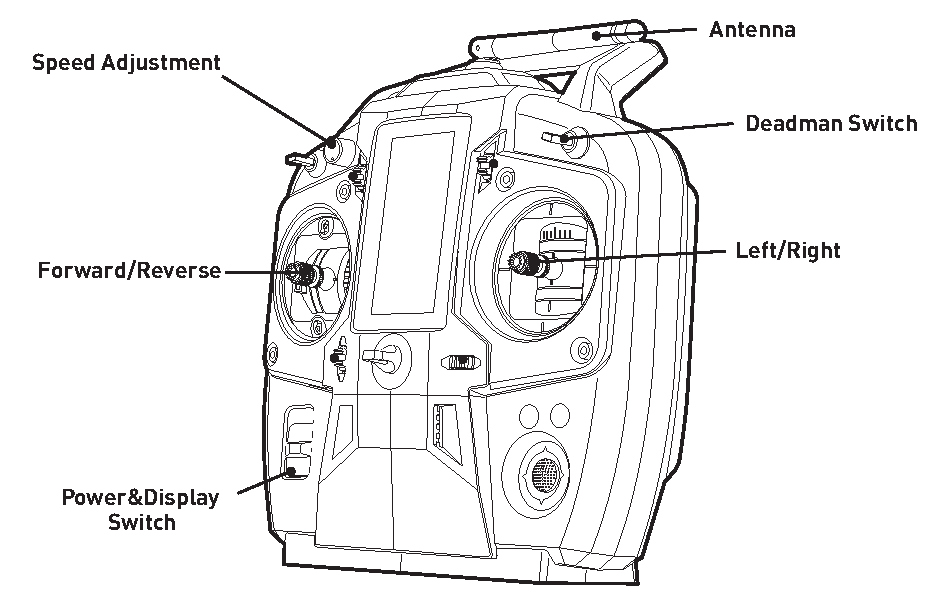
\includegraphics[width=1.0\linewidth]{graphics/futaba.png}
  \caption{Futaba Radio Transmitter}
  \label{futaba}
\end{figure}

\begin{figure}[!h]
  \centering
  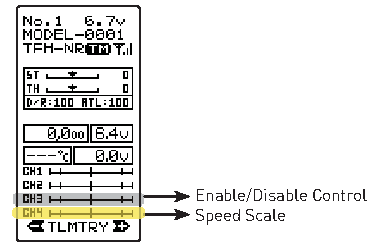
\includegraphics[width=1.0\linewidth]{futaba-screen.pdf}
  \caption{Futaba Radio Transmitter Screen}
  \label{futaba-screen}
\end{figure}

If you’re not seeing any action, check Contact on \autoref{contact} to get in touch with support.


\pagebreak[4]

\subsection{Body Lights}

Warthog includes four RGB body lights, stacked in a pair on each corner of the chassis. These lights express system status according to \autoref{bodylights}. In the absence of one of the low-level conditions, they can be commanded from ROS to display indications from autonomy or other higher-level software.


\bgroup
\def\arraystretch{1.2}%
\begin{table}[h]
  \centering
  \begin{tabular}{>{\columncolor{lightgrey}}>{\raggedright}m{.25\textwidth} p{.7\textwidth}} \hline

  Solid red & The MCU is not in contact with the computer. That is, the rosserial connection is not active. This condition will be seen briefly on startup while Warthog's computer is booting up. If it persists, or is seen after initialization, either the base node on the PC has crashed, the network switch has failed, or a serious MCU error has occurred. If you suspect one of these conditions, please contact our support team. \\ \hline

  Red flashing & Stop circuit is broken. Twist the mushroom buttons to ensure that they're unlatched, and check any external stop hardware, if present. \\ \hline

  Flashing yellow & Motor drivers not yet ready to drive. The motors have a brief initialization sequence which must complete after a stop condition clears before they are ready to drive. If this condition persists, please contact our support team. \\ \hline

  Headlights/taillights & When Warthog is ready to drive, the front will change from red to white. The intensity of the head and tail lights will increase slightly when actually in motion. This is the status which may be overridden by publishing your own light patterns to the cmd\_lights ROS topic. \\ \hline

  \end{tabular}
\newline
\caption{Warthog Body Light Indications}
\label{bodylights}
\end{table}
\egroup

\pagebreak[4]


\subsection{Wireless Access}

To get the Warthog connected to your local wifi, you must first access the internal computer using a wired connection. Connect to one of the network ports with a standard ethernet cable. Now, set your laptop’s ethernet port to a static IP such as \lstinline{192.168.131.123}, and connect via SSH to \lstinline{administrator@192.168.131.1}. The default password is \lstinline{clearpath}.

Now that you're connected via SSH over a wired connection, you can setup Warthog to connect to a local wifi network.  To do this, you will use the wireless interface configuration daemon (WICD) - a preinstalled network manager.

In a terminal window, execute the following command:

\begin{lstlisting}
wicd-curses
\end{lstlisting}

You should see a browsable list of networks which the robot has detected. Use arrow keys to select the one you would like to connect to, and then press the right arrow to configure it. You can enter your network’s password near the bottom of the page, and note that you must select the correct encryption scheme; most modern networks use WPA1/2 Passphrase, so if that’s you, make sure that option is selected. You also likely want to select the option to automatically reconnect to this network, so that Warthog will be there for you on your wireless automatically in the future.

When you’re finished, press \textbf{F10} to save, and then \textbf{C} to connect.  Warthog is now connected to wifi!

While you're still wired to Warthog, you'll need to identify the IP address of Warthog's wireless connection.

In a terminal window, execute:

\begin{lstlisting}
ifconfig
\end{lstlisting}

A list of network connections will be displayed within the terminal.  Locate the wireless network and make note of its IP address. Now that you know Warthog's wireless IP address, you may now exit the ethernet SSH session by executing \lstinline{exit}.

Remove the ethernet cord from the Warthog.   Now you can SSH into Warthog over the wireless network.  To do so, execute:

\begin{lstlisting}
ssh administrator@<IP_OF_Warthog>
\end{lstlisting}

SSH sessions allow you to control Warthog's internal computer.  You can do various things such as download packages, run updates, add/remove files, transfer files etc.

\subsection{Remote ROS Connectivity}

Now that Warthog is on the wireless network, you can access it via SSH or as a remote ROS master. Note that in the default configuration, the background ROS process running on Warthog launches with the \lstinline{robot_upstart} package. This is configured to set the \lstinline{ROS_HOSTNAME} environment variable to the Warthog PC's hostname.

If your network resolves hostnames properly, connecting should be a matter of executing the following two lines in your desktop (or sourcing a script containing these lines):

\begin{lstlisting}
export ROS_MASTER_URI=http://cpr-warthog:11311     # Your robot's hostname
export ROS_IP=192.168.131.1                        # Your computer's wireless IP address
\end{lstlisting}

If your network doesn't resolve hostnames, you may need to add the following line to your \lstinline{/etc/hosts} file:

\begin{lstlisting}
192.168.131.1 cpr-warthog                         # The robot's wireless IP address.
\end{lstlisting}

Once everything is set up correctly, try running \lstinline{rostopic list}. This will verify that your machine can see the robot's ROS master. Then try running \lstinline{rostopic echo /mcu/status}. This will verify that the robot PC can see your machine in order to stream topics to it.

Please contact Clearpath Support if guidance is required in selecting and executing a remote access strategy.
For more general details on how ROS works over TCP with multiple machines, please see:

\url{http://wiki.ros.org/ROS/Tutorials/MultipleMachines}

For help troubleshooting a multiple machines connectivity issue, see:

\url{http://wiki.ros.org/ROS/NetworkSetup}

\subsection{Visualizing Warthog}

To command or observe Warthog from your desktop computer, first set up a basic ROS installation.  See the following page for details:

\url{http://wiki.ros.org/melodic/Installation/Ubuntu}

When your ROS install is set up, install the Warthog desktop packages:

\begin{lstlisting}
sudo apt-get install ros-melodic-warthog-desktop
\end{lstlisting}

Once your remote access to Warthog's ROS master is configured (as above), you can launch rviz, the standard ROS robot visualization tool:

\begin{lstlisting}
roslaunch warthog_viz view_robot.launch
\end{lstlisting}

From within rviz, you can use interactive markers to drive Warthog. You can visualize its published localization estimate, and you can visualize any attached sensors which have been added to its robot description XML (URDF).

\pagebreak[4]

From your desktop, you can also launch the standard RQT Robot Monitor. This will report the diagnostic output from Warthog's self-monitoring capabilities, as shown in \autoref{robotmonitor}:

\begin{lstlisting}
rosrun rqt_robot_monitor rqt_robot_monitor
\end{lstlisting}

\begin{figure}[!htb]
  \centering
  \includegraphics[width=0.70\linewidth]{graphics/rqt_robot_monitor.png}
  \caption{Robot Monitor}
  \label{robotmonitor}
\end{figure}


\subsection{Drive Train}

The Warthog has the ability to be put into neutral which is controlled be the four levers (two per side) in the rockers.  The lever can be seen in \autoref{lever}.  Use the bolts to restrict the lever from moving as down in \autoref{drivetrain-n} where the drivetrain is in neutral.  The grove for the neutral position is marked with white and the bolt is also marked.  Pull the handle on the lever to move it into gear which can be seen in \autoref{drivetrain-g}.  Ensure the lever is in the green grove.  If the lever is difficult to move, rock the Warthog back and forth.  Do not try to force the lever to move.

\begin{figure}[!htb]
  \centering
  \includegraphics[width=0.25\linewidth]{graphics/drivetrain.png}
  \caption{Drivetrain lever}
  \label{lever}
\end{figure}


\begin{figure}[!htb]
  \centering
  \includegraphics[width=0.75\linewidth]{graphics/drivetrain-neutral.png}
  \caption{Drivetrain in Neutral}
  \label{drivetrain-n}
\end{figure}


\begin{figure}[!t]
  \centering
  \includegraphics[width=0.75\linewidth]{graphics/drivetrain-gear.png}
  \caption{Drivetrain in Gear}
  \label{drivetrain-g}
\end{figure}





\section{Payload Integration Guide}

If you want to attach custom hardware to Warthog, you will have to take care of mechanical mounting, electrical supply, and software integration.  This section aims to equip you with respect to these challenges.

\subsection{System Architecture}

Like most robotic systems, Warthog has an onboard PC coupled to a custom microcontroller board. The microcontroller board handles IO, system and battery monitoring, and provides an interface to the CAN-controlled motor drivers. See the diagram in \autoref{systemarchitecture} for more details.

\begin{figure}[!htb]
  \centering
  \includegraphics[width=1.0\linewidth]{warthog-logic-conn.pdf}
  \caption{System Architecture}
  \label{systemarchitecture}
\end{figure}

Using ROS to interface with the Warthog, the ROS API described in \autoref{tab:rosapi} can be used and the node connections can be seen in \autoref{fig:rqt-graph}

\bgroup
\begin{table}[htp]
\begin{tabular}{  l  l  p{7cm} }
\hline
Topic & Message Type & Purpose \\ \hline

\lstinline!/cmd_vel! & \lstinline!geometry_msgs/Twist! &
Input to Warthog's kinematic controller. Publish here to make Warthog go. \\ \hline
\lstinline!/odometry/filtered! & \lstinline!nav_msgs/Odometry! &
Published by \lstinline!robot_localization!, a filtered localization estimate based
on wheel odometry (encoders) and  integrated IMU. \\ \hline

\lstinline!/imu/data! & \lstinline!sensor_msgs/IMU! &
Published by \lstinline!imu_filter_madgwick!, an orientation estimate based on Warthog's
internal gyroscope, accelerometer, and magnetometer. \\ \hline

\lstinline!/status! & \lstinline! warthog_msgs/Status! &
Low-frequency status data for Warthog's systems. This information is republished in human
readable form on the \lstinline!diagnostics! topic and is best consumed with the Robot
Monitor. \\ \hline

\lstinline!/cmd_lights! & \lstinline! warthog_msgs/Lights! &
Input to controlling the Warthog's body lights when not in an error state. \\ \hline


\lstinline!/SIDE/speed! & \lstinline! std_msgs/Float64! &
Input velocity for each motor where \textit{SIDE} is either left or right.  This should not be published to directly, commands from \lstinline!/cmd_vel! will be converted to this.\\ \hline

\lstinline!/SIDE/status/speed! & \lstinline! std_msgs/Float64! &
Reported velocity from each motor's encoder where \textit{SIDE} is either left or right. \\ \hline

\lstinline!/SIDE/status/fault! & \lstinline! std_msgs/Bool! &
Reported state from each motor controller where \textit{SIDE} is either left or right. \\ \hline

\lstinline!/SIDE/status/motor_temperature! & \lstinline! std_msgs/Int32! &
Reported temperature from each motor controller where \textit{SIDE} is either left or right. \\ \hline

\end{tabular}
\caption{Warthog ROS API Topics}
\label{tab:rosapi}
\end{table}
\egroup

\begin{figure}[!htb]
  \centering
  \includegraphics[width=0.75\linewidth]{graphics/rqt-graph.png}
  \caption{Warthog Node and Topic connections}
  \label{fig:rqt-graph}
\end{figure}
\clearpage

\pagebreak[4]
\subsection{Mechanical Mounting}
\label{mechanical}

The payload integration area can be used to mount external payloads on top of the Warthog.


\subsubsection{Payload Integration Guidelines}

\begin{itemize}[nolistsep]

\item 27.75” is the maximum allowed width of any installed payload (this assumes that the payload is also centered across the width of the UGV chassis.

\item  No part of the payload may extend over the sheet metal housings of the drive units or into the small (~2”) gaps between the chassis and drive units. Damage to both the UGV and the payload WILL result.

\item  The chassis has a removable access cover measuring ~46.25” x 26.25”. This access cover is supported underneath by two adjustable cross members. Regardless of payload, it is imperative that both cross members remain installed (approximately evenly spaced) to provided required support to the access cover. Consider that any payload installed above the top deck will prevent access to the chassis through the access cover, without first removing the installed payload.

\item  The rotation of the suspension differential link in the horizontal plane will allow the payload to extend beyond the chassis top deck in both fore and aft locations. The amount of this payload extension (overhang) is dependent on several factors, including the weight and method of attachment of the payload as well as the terrain in which the UGV will operate. Ensure that the amount of overhanging payload allows the UGV to operate safely and does not contact the terrain, especially when crossing steep and/or deep gullies.

\item  The available internal chassis volume is approximately 17.5” long x 26” wide x 9.5” high. This space is located at the center of the chassis between two battery packs. Consider that anything placed inside the chassis MUST be secured as to not move or shift during UGV operation. Any payload secured inside the chassis must also be insulated from coming into contact with the battery wiring and terminals.

\end{itemize}




\begin{warning}[]
Permanent damage resulting from custom modifications to the mounting plate is not covered under warranty and may not be supported by Clearpath Support.  Please contact our support team if you require assistance or have any questions relating to custom modifications.
\end{warning}


\pagebreak[4]
\subsection{Electrical Integration}
\label{electrical}

The user power receptacles located in the User Panel are capable of supplying 12Vdc, 24Vdc, and unregulated battery voltage (approximately 48Vdc) for powering Warthog's payloads. See \autoref{userpower} for a labeled illustration and \autoref{userpowerpinout} for the pin assignments. Ensure you select a contact that's appropriate for the gauge of wire used.

The electrical system for the chassis can be seen in \autoref{elec-chassis}. Additionally, left and right drive units electrical system is described in \autoref{elec-left} and \autoref{elec-right} respectively.





\begin{figure}[!h]
  \centering
  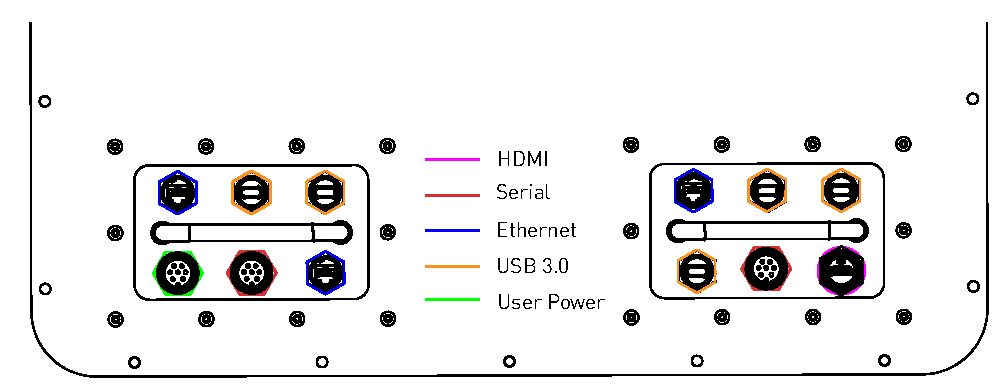
\includegraphics[width=1.0\linewidth]{graphics/User_Panel_Labeled.png}
  \caption{Warthog User Panel}
  \label{userpower}
\end{figure}


\begin{warning}[Risk of Fire]
For continued protection against risk of fire, always replace fuses only with those of the same type and rating.
\end{warning}


\begin{figure}[!htb]
  \centering
  \includegraphics[width=1.0\linewidth]{graphics/Breakout_pinouts.png}
  \caption{Warthog Power User Connector Pinout}
  \label{userpowerpinout}
\end{figure}

\pagebreak
\begin{figure}[!htb]
  \centering
  \includegraphics[width=0.9\linewidth]{elec-chassis.pdf}
  \caption{Warthog Chassis Electrical System}
  \label{elec-chassis}
\end{figure}

\begin{figure}[!htb]
  \centering
  \includegraphics[width=0.9\linewidth]{elec-left.pdf}
  \caption{Warthog Left Drive Unit Electrical System}
  \label{elec-left}
\end{figure}

\begin{figure}[!htb]
  \centering
  \includegraphics[width=0.9\linewidth]{elec-right.pdf}
  \caption{Warthog Right Drive Unit Electrical System}
  \label{elec-right}
\end{figure}




\subsection{Software Integration}

ROS has a large ecosystem of sensor drivers, some of which include pre-made URDF description and even simulation configurations.  Please see the following page on the ROS wiki for a partial list:

\url{http://wiki.ros.org/Sensors}

For the best experience, consider purchasing supported accessories from Clearpath Robotics for your Warthog. This will include simulation, visualization, and driver support for those accessories.  However, we will happily help you get started with integrating your own devices as well.

\section{Maintenance}

\subsection{Battery \& Charging}

\subsubsection{General}

Warthog contains 48V lead-acid or lithium-ion battery packs. Each battery pack consists of four 12V lead-acid or lithium-ion batteries.

Battery configuration may vary with each unit. In order to maximize performance, it's important to ensure that the battery level across each set of lead-acid or lithium-ion batteries is within 0.1-0.2V of each other. If the battery packs exceed this tolerance, it's advised to charge them to within tolerance before wiring these packs
in parallel. The overall battery life will vary depending upon the usage of the unit.

Always exercise caution and observe the following safety practices when connecting, disconnecting or handling batteries:

\begin{itemize}[nolistsep]
  \item Batteries are high voltage, high current
  \item Battery packs must be properly fastened down to ensure they do not move when the Warthog is in operation.
  \item Ensure that the battery packs are evenly distributed throughout the Warthog to maximize stability.
  \item Battery levels on the unit should be checked on a regular basis.  It's important to maintain the battery voltage at a suitable level for proper operation.
  \item When additional battery packs are added to the system, it's important to connect the positive terminal first to the main power of the Warthog before connecting ground.
  \item When installing additional battery packs, disconnect the ground on all battery packs presently in the unit before connecting the positive terminal of the new battery packs.
\end{itemize}

\subsection{Lithium Battery Upgrade}
The following section applies to units with the lithium battery upgrade. The lithium battery upgrade has the added benefits of a longer run time, lighter weight and a longer lifespan. With lithium battery arrays it is especially important to charge the vehicle after use and periodically if it sits for a long period of time, as the batteries need to balance for optimum performance.

The Warthog array is configured in a 4 series by 3 parallel configuration for a total of 12 batteries, therefore inter-battery balancing is critical. Due to differences in the internal series resistance between batteries, the individual state of charge of each battery will vary with respect to the other batteries. When in the bulk charging phase there is no chance to equalize the charge level of each individual battery, thus a balancing phase is required. This balancing (sometimes referred to as equalization) occurs after the main bulk charging phase, and is a phase where lower current from the charger at a constant voltage is applied to the array. The individual battery modules will internally balance themselves (internal cells), but the overall series string will need time to balance between battery modules. The charger should be allowed to remain on and connected for a period of a few hours after the bulk phase. Depending on the imbalance between batteries, this could range anywhere from 2 to 8 hours.

Quick bulk charges can be done if uptime is required, but it is highly recommended to allow for a complete balancing cycle every third charge, minimally, to keep the array well balanced and at peak performance. Not following this recommendation will result in degraded performance and could possibly end in damage to one or more of the batteries prematurely.

The status of each battery can be check in ROS through one of the robots topics. This topic is the '/nec\textunderscore node/modules' topic. To view this topic run the following command:

\begin{lstlisting}
rostopic echo /nec_node/modules
\end{lstlisting}

This will begin to stream the data from all 12 batteries. Press 'ctrl+c' to end the streaming of the topic. Data like the remaining battery capacity, cell voltages, individual current output and much more can be found here. It should be noted that there is currently a known issue where one or more of the batteries does not publish its data right away or will intermittently cut out. If this happens during startup or when launching ROS, this topic will not show up. This can sometimes be fixed by restarting ROS or by restarting the robot. This topic has no effect on the vehicles operation in any way! It is there for the user to monitor battery health both instantaneously and over the lifetime of the batteries. To check if the topic has launched, run the following command:

\begin{lstlisting}
rostopic list
\end{lstlisting}

This will show all topics currently running on the robot. If the topic is not found then the next thing would be to restart ROS with this command:

\begin{lstlisting}
sudo systemctl restart ros
\end{lstlisting}

Enter the password 'clearpath' if prompted. Now you may check again if the topic has launched. This does not guarantee it will and if not then you will have to try again later. For more information on this known issue, please contact Clearpath Robotics any time. We are actively working with the manufacturer to resolve this issue.



\subsubsection{Long-term Storage}

When storing Warthog for long periods of time, it's important to properly maintain the batteries to fully maximize their life.  Consider one of the following two procedures when placing Warthog in long-term storage:

\begin{itemize}[nolistsep]
  \item Fully charge Warthog, turn it off and put it into storage.  Once a week, connect power to the charger and allow the charger to top up the battery for an hour or so.
  \item Fully charge Warthog, turn it off and put it into storage, but leave the charger connected and powered the entire time Warthog is in storage.  The charger will monitor the battery and will automatically charge it up as needed.
\end{itemize}


Please contact Clearpath Robotics for additional information about Warthog's battery pack.

\subsection{Track Drive Upgrade}
If your unit came equipped with the track drive upgrade, please keep the following considerations in mind

\begin{itemize}
\item The track drive drive units pull considerably more current to operate. It is advised to operate a track drive Warthog at reduced speeds, either through ROS commands or by reducing the speed scale when operating with the Futaba controller.
\item Due to the increased drive current, expect lower battery life than a wheeled Warthog. It is recommend to drive at reduced speeds to increase battery life.
\item It is possible to trigger an over current error in the motor controller by increasing speed drastically shortly after resetting a stop condition. The system's body lights will seem as if the unit is ready to drive, however it will not respond to drive commands. To clear this state, simply cycle another stop condition, and reduce the ramp up speeds.
\end{itemize}

\section{Contact}
\label{contact}

Clearpath is committed to your success with Warthog. Please get in touch with us and we’ll do our best to get
you rolling again quickly: \url{support@clearpathrobotics.com}.

To get in touch with a salesperson regarding Warthog or other Clearpath Robotics products, please email
\url{sales@clearpathrobotics.com}.

If you have an issue that is specifically about ROS and is something which may be of interest to the broader
community, consider asking it on \url{answers.ros.org}. If you don’t get a satisfactory response, please ping us and
include a link to your question as posted there. If appropriate, we’ll answer in the ROS Answers context for
the benefit of the community.

\appendix

\thispagestyle{empty}
\includepdf[pages=1-4]{charger.pdf}
\thispagestyle{empty}

\end{document}
